\section{Auswertung}
\subsection{Untersuchung eines Reflexklytrons}
Die Messwerte der Untersuchung drei verschiedener Moden auf einem Oszilloskop sind
in Tabelle \ref{tab:reflex} eingetragen.
\begin{table}
  \centering
  \begin{tabular}{c c c c c c}
    \toprule
    {Mode} & {$U_0$\,/\,V} & {$U_1$\,/\,V} & {$U_2$\,/\,V} & {$A_0$\,/\,V} & {$f_0$\,/\,MHz} \\
    \midrule
    1 & 60 & 50 & 70 & 0,9 & 9015 \\
    2 & 100 & 90 & 110 & 1,3 & 9007 \\
    3 & 150 & 140 & 170 & 2,5 & 9001 \\
    \bottomrule
  \end{tabular}
  \caption{Messwerte für die Reflektorspannungen mit der jeweiligen Amplitude und Frequenz}
  \label{tab:reflex}
\end{table}
\newline
Aus den Messwerten kann eine Regression der Form
\begin{align*}
    A(U) = xU^2 + yU+ z
\end{align*}
durchgeführt werden. Diese ist in Abbildung \ref{fig:regression} zu sehen.
\begin{figure}
  \centering
  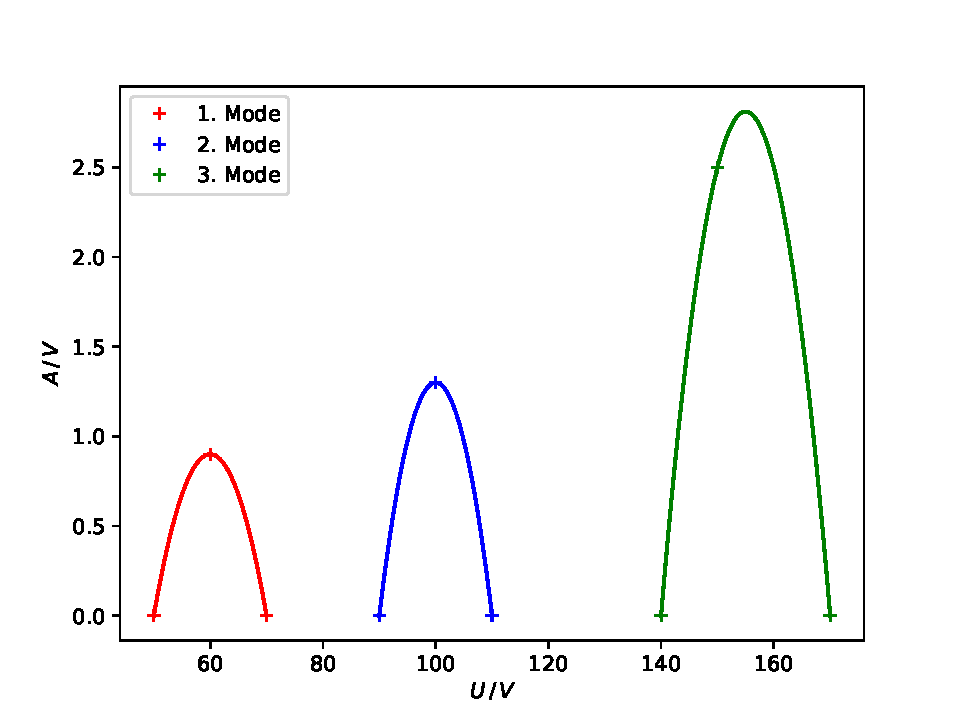
\includegraphics[width = 12 cm]{moden.pdf}
  \caption{Graphen der drei Moden}
  \label{fig:regression}
\end{figure}
\newpage
Die daraus resultierenden Parameter sind in Tabelle \ref{tab:params} aufgetragen.
\begin{table}
    \centering
    \begin{tabular}{c c c}
        \toprule
        {$x$\,/\,$\frac{1}{V}$} & {$y$} & {$z$\,/\,V}\\
        \midrule
        -0,009 & 1,080 & -31,500 \\
        2,600 & -0,013 & -128,700 \\
        3,875 & -0,125 & -297,450 \\
        \bottomrule
    \end{tabular}
    \caption{Fitparameter der Reflektorspannungen}
    \label{tab:params}
\end{table}
\newline
Für die elektronische Abstimmung des Reflexklytrons sind die Messwerte in Tabelle \ref{tab:elektronisch} zu sehen.
\begin{table}
    \centering
    \begin{tabular}{c c}
        \toprule
        {$U_0$\,/\,V} & {$f_0$\,/\,MHz} \\
        \midrule
         235 & 9001 \\
         230 & 8985 \\
         250 & 9021 \\
        \bottomrule
    \end{tabular}
    \caption{Messwerte der elektronischen Abstimmung}
    \label{tab:elektronisch}
\end{table}
\newline
Die Bandbreite $\symup\Delta f$ berechnet sich nach
\begin{align*}
    \Delta f = f^{\shortmid} -f^{\shortmid\shortmid} = 20\mathrm{MHz}.
\end{align*}
\newline
Für die Abstimmempfindlichkteit ergibt sich mithilfe der zuvor berechneten Bandbreite
\begin{align*}
    E = \frac{f^{\shortmid} - f^{\shortmid\shortmid}}{U^{\shortmid} - U^{\shortmid\shortmid}} = 1,33 \,\frac{\su{MHz}}{\su{V}}.
\end{align*}

\newpage
\subsection{Messung von Frequenz, Wellenlänge und Dämpfung}
Die Messwerte sind in Tabelle \ref{tab:frequenz} dargestellt.
\begin{table}
    \centering
    \begin{tabular}{c c c c c}
        \toprule
        {$f$\,/\,MHz} & {1. Minimum\,/\,mm} & {2. Minimum\,/\,mm} & {$\lambda_g$\,/\,mm} & {$a$\,/\,mm}\\
        \midrule
        8952 & 72,6 & 97,5 & 43,7 & 21,85\\
        \bottomrule
    \end{tabular}
    \caption{Messreihe zur Bestimmung der Frequenz}
    \label{tab:frequenz}
\end{table}
\newline
Der Abstand $a$ ist dabei genau der Abstand zwischen den beiden Minima.
Aus diesem wird die Hohlwellenlänge $\lambda_g$ berechnet, welche genau dem doppelte Abstand $a$ entspricht.
\newline
Mit Formel \ref{eqn:1} ergibt sich die Frequenz $f = 9701,84$\,MHz.
\newline
In Tabelle \ref{tab:swr} sind die Messergebnisse für die Dämpfung zu sehen.
Bei der Mikrometereinstellung sind die Werte auf 2,5\,mm normiert.
\begin{table}
    \centering
    \begin{tabular}{c c c c}
        \toprule
        {SWR-Meter Ausschlag\,/\,dB} & {Mikrometereinstellung\,/\,mm} & {Dämpfung\,/\,dB} & {Abweichung}\\
        \midrule
         0 & 0,00 & 0,0 & 0\% \\
         2 & 0,50 & 1,0 & 200\% \\
         4 & 0,70 & 1,5 & 267\% \\
         6 & 1,00 & 2,0 & 300\% \\
         8 & 1,15 & 3,0 & 267\%\\
         10 & 1,25 & 4,3 & 233\%\\
        \bottomrule
    \end{tabular}
    \caption{Messergebnisse der Dämpfung}
    \label{tab:swr}
\end{table}
\newline
In Abbildung \ref{fig:dämpfung} ist die Dämpfungskurve dargestellt.
\begin{figure}
  \centering
  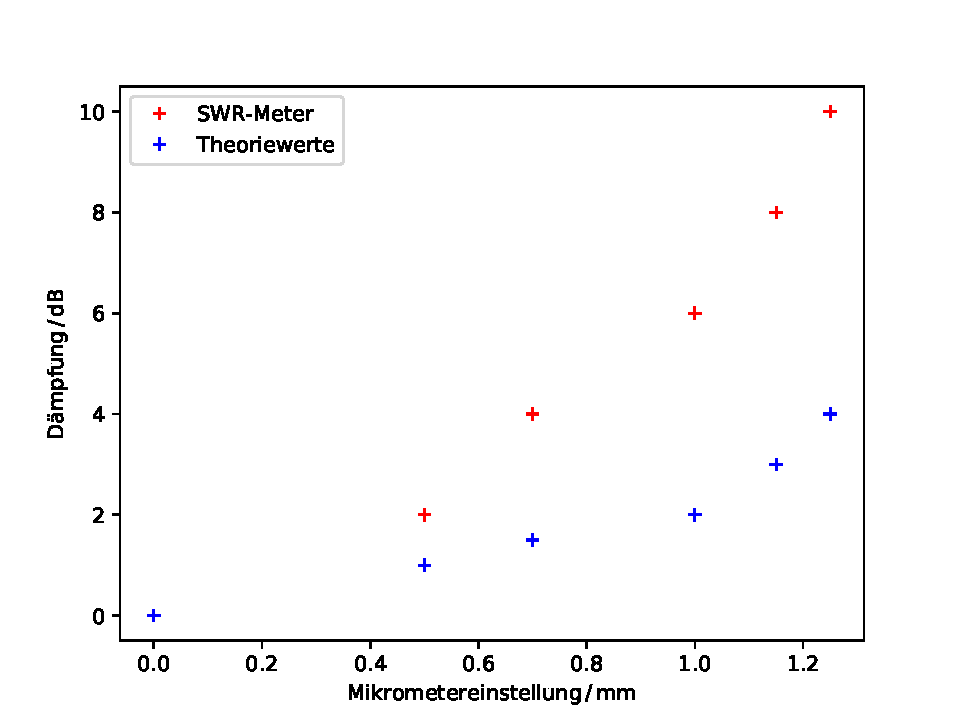
\includegraphics[width = 12 cm]{dämpfung.pdf}
  \caption{Vergleich der experimentellen und theoretischen Werte der Dämpfungskurve}
  \label{fig:dämpfung}
\end{figure}

\newpage
\subsection{Stehwellenmessung}
Zur Bestimmung der Stehwellenmessungen werden die drei möglichen Methoden durchgeführt.
Die resultierenden Messergebnisse sind aus Tabelle \ref{tab:swr} für die SWR-Methode,
in Tabelle \ref{tab:3dB} für die 3dB-Methode und in Tabelle \ref{tab:abschwächer} für die
Abschwächer-Methode zu entnehmen.
\begin{table}
    \centering
    \begin{tabular}{c c c}
        \toprule
        {Sondentiefe\,/\,V} & {SWR-Meter Ausschlag} \\
        \midrule
         3 & 1,430 \\
         5 & 1,625 \\
         7 & 2,400 \\
         9 & 4,000 \\
        \bottomrule
    \end{tabular}
    \caption{SWR-Meter-Methode}
    \label{tab:swr}
\end{table}
\newline
Bei der 3dB-Methode lässt sich das SWR mithilfe von Formel \ref{eqn:2} berechnen.
\begin{table}
    \centering
    \begin{tabular}{c c c c c c}
        \toprule
        {$d_1$\,/\,mm} & {$d_2$\,/\,mm} & {1. Minimum\,/\,mm} & {2. Minimum\,/\,mm} & {$\lambda_g$} & {SWR}\\
        \midrule
         77 & 54 & 69 & 72 & 27,2 & 4,88 \\
        \bottomrule
    \end{tabular}
    \caption{3\,dB-Methode}
    \label{tab:3dB}
\end{table}
\begin{table}
    \centering
    \begin{tabular}{c c c c}
        \toprule
        {$A_1$\,/\,dB} & {$A_2$\,/\,dB} & {$|A_2-A_1|$\,/\,dB} & {SWR$=\frac{\Delta A}{2}$} \\
        \midrule
        20 & 27,14 & 7,14 & 3,57 \\
        \bottomrule
    \end{tabular}
    \caption{Abschwächer-Methode}
    \label{tab:abschwächer}
\end{table}

\section{Diskussion}
Die Bestimmung der Messwerte mithilfe des SWR-Meters führte während der Durchführung
zu einigen Ungenauigkeiten, da dieses auf kleinste Bewegungen im Raum reagierte.

Der zu erwartenene Anstieg der Amplituden bei steigender Reflektorspannung ist in
der Diagramm der 3 Moden gut zu erkennen. Jedoch stimmt bei der 3. Mode das Maximum der Parabel
nicht mit dem gemessen Maximum überein. Der Grund dafür könnte sein, dass die Einsattelung
nicht genau mit dem Oszilloskop erkennbar war.

Die Ergebnisse für die experimentell und theoretisch bestimmte Frequenz
ist in Tabelle \ref{tab:f-Vergleich} zu sehen.
\begin{table}
    \centering
    \begin{tabular}{c c c}
        \toprule
        {$f_0\,/\,$MHz} & {$f_{\su{berechnet}}\,/\,$MHz} & {Abweichung} \\
        \midrule
        8952 & 9701,84 & 7,7\% \\
        \bottomrule
    \end{tabular}
    \caption{Vergleich der Frequenzen}
    \label{tab:f-Vergleich}
\end{table}
\newline
Die prozentuale Abweichung liegt bei 7,7\%. Diese Abweichung lässt sich durch das schwierigere Auffinden
zweier Minima erklären.

Bei der Messung der Dämpfung liegt die prozentuale Abweichung in einem hohen Bereich von 200-30\%.
Diese ist auch in Abbildung \ref{fig:dämpfung} zu sehen. Die gemessenen Werte weichen sehr stark von
den Theoriewerten ab. Hier ist schon während des Versuchs aufgefallen, dass die Messwerte so nicht stimmen können und sich ein systematischer
Fehler eingeschlichen hat, der allerdings nicht behoben werden konnte. Deshalb ist die Messreihe eher zu
vernachlässigen.

Die Ergebnisse für die drei verschiedenen Methoden der Stehwellenmessung sind in Tabelle \ref{tab:SWR-Vergleich}
dargestellt.
\begin{table}
    \centering
    \begin{tabular}{c c c}
        \toprule
        {SWR-Meter-Methode} & {3\,dB-Methode} & {Abschwächer-Methode} \\
        \midrule
         4 & 4,8 & 3,57\\
        \bottomrule
    \end{tabular}
    \caption{Vergleich der unterschiedlichen Methoden}
    \label{tab:SWR-Vergleich}
\end{table}
\newline
Es fällt auf, dass die Werte alle in derselben Größenordnung liegen, aber besonders der Wert der SWR-Meter-Methode
deutlich von dem Wert der Abschwächer-Methode abweicht. Auch hier könnte die fehlerhaft verwendete
Dämpfung zu der Ungenauigkeit beigetragen haben.
